
\section{Classificador \textit{Naïve Bayes}.}
\label{subsec::cred_nb}

Nessa seção, explicamos o funcionamento do algoritmo \textit{Naïve Bayes} original. É importante termos em mente a versão original do mesmo para que possamos compará-la à versão na qual a credibilidade é incorporada (ver Seção~\ref{subsubsec::nb_cred}). Referências mais detalhadas do \textit{Naïve Bayes} podem ser encontradas em \cite{DHS01} e \cite{Manning08}.

De uma maneira sucinta, porém prática, podemos utilizar os seguintes passos para definir o classificador \textit{Naïve Bayes}:

\begin{enumerate}
    \item Cada um dos exemplos do conjunto de treinamento pode ser visto como uma tupla $D$-dimensional, $X$ = ($x_1$, $x_2$, $x_3$, ..., $x_D$), onde $x_i$ é o valor referente ao atributo $A_i$ no exemplo $X$. É importante ressaltar que para um atributo $A_i$, podemos ter valores distintos de $x_i$ nos vários exemplos de treino. Tipicamente, em um problema de classificação com atributos numéricos, $x_i$ pode assumir qualquer valor real. Já em um problema de classificação categórico, $x_i$ pode assumir uma faixa controlada de valores discretos. Em classificação de documentos, por exemplo, $x_i$ pode ser qualquer valor inteiro natural, representando o número de vezes que temos um termo $A_i$ em um documento $X$. Vale a pena lembrar também que podemos ter a coexistência de atributos numéricos e categóricos em uma mesma base de dados.
    

    \item Suponha que existem \textit{M} classes, $c_1$, $c_2$, ..., $c_\textit{M}$, formando o conjunto de possíveis classes $\mathbb{C}$. Dado um determinado exemplo $X$, o classificador Bayesiano prevê que $X$ pertence à classe que tiver a maior probabilidade a \textit{posteriori} $P(c_j|X)$. Ou seja, o classificador \textit{Naïve Bayes} diz que $X$ pertence a $c_j$, se e somente se:
        
\begin{equation}\label{eqn::max_pcgivenx}
   P(c_{j}|X) > P(c_{k}|X) \;\;\;\;\;\forall k,\; 1 \le k \le M, \; k \not= j,
\end{equation}
onde $P(A|B)$ é um valor real entre 0.0 e 1.0 que define a probabilidade do evento A ser verdadeiro, dado que o evento B ocorreu. No caso, podemos interpretar a expressão $P(c_j|X)$ como a probabilidade da classe correta ser $c_j$ dado o exemplo $D$-dimensional $X$ = ($x_1$, $x_2$, ..., $x_D$).

    \item Necessitamos, portanto, de uma forma de calcular a probabilidade a \textit{posteriori} $P(c_j| X)$, que pode ser definida pelo teorema de Bayes como:
\begin{equation}\label{eqn::bayes}
   P(c_{j}|X) = \frac{P(X|c_j) \times P(c_j) }{P(X)}
\end{equation}

    \item Da Equação~\ref{eqn::bayes} temos que $P(c_j)$ pode ser obtida simplesmente calculando a proporção de exemplos da classe $c_j$ que temos em nosso conjunto de treinamento. Além disso, a probabilidade $P(X)$ é uma constante independente da classe e, por isso, não precisamos calculá-la.
       
    \item Obter $P(X|c_j)$ é uma tarefa extremamente cara computacionalmente. Porém podemos utilizar a premissa ``ingênua'' 
    %\footnote{O nome do algoritmo Naïve Bayes provém dessa premissa simplificadora.} 
    de que os valores dos atributos de um exemplo $X$ são condicionalmente independentes um dos outros, dada uma certa classe. Logo,

\begin{equation}\label{eqn::classindependence}
   P(X|c_{j}) = \prod^{D}_{i=1}{P(x_i|c_j) }
\end{equation}

\item O valor de cada termo $P(x_i|c_j)$ da Equação~\ref{eqn::classindependence} é usualmente calculado de forma diferente caso o atributo $A_i$ seja categórico, textual ou numérico. A seguir mostramos as formas mais comuns vistas na literatura:
    \begin{itemize}

        \item Caso $A_i$ seja categórico, então $P(x_i|c_j)$ é o número de exemplos no treinamento que pertencem a classe $c_j$, nos quais o valor de $A_i$ é $x_i$, dividido pelo número de exemplos da classe $c_j$ no treino:

    \begin{equation}\label{eqn::nbcattexto}
        P(x_i|c_j) = \frac{ F_{x_{i}c_{j}} }{ F_{c_{j}} },
    \end{equation}
        onde $F_{x_{i}c_{j}}$ é o número de vezes que temos o termo $x_i$ nos exemplos de treino da classe $c_j$ e $F_{c_{j}}$ é o número de exemplos de treino da classe $c_j$.
        
        \item Caso $A_i$ seja textual, temos uma versão ligeiramente diferente que pode ser expressa na seguinte fórmula:

    \begin{equation}\label{eqn::nbcattexto}
        P(t_i|c_j) = \frac{ F_{t_{i}c_{j}} }{ \sum\limits^{D}_{k = 1} { } F_{t_{k}c_{j}} },
    \end{equation}
        onde $F_{t_{i}c_{j}}$ é o número de vezes que temos o termo $t_i$ nos exemplos de treino da classe $c_j$ e $D$ é o número de atributos existentes (tamanho do vocabulário conhecido).

        \item Caso $A_i$ seja um atributo numérico, tipicamente um valor real, então assumimos que o valor $x_i$ do atributo $A_i$ é dado por uma distribuição Gaussiana de média $\mu_i$ e desvio padrão $\sigma_i$ e podemos usar a seguinte fórmula para calcular $P(x_i|c_j)$:
    \begin{eqnarray}\label{eqn::nbnumerico}
        P(x_i|c_j) & = & g(x_i, \mu_{ic_j}, \sigma_{ic_j})  \\
        g(x, \mu, \sigma) & = & \frac {1} { \sqrt{2\pi\sigma} } e^{ -\frac{(x-\mu)^2}{2\sigma^2}  } 
    \end{eqnarray}
        onde $\mu_{ic_j}$ e $\sigma_{ic_j}$ são a média e o desvio padrão dos valores de $A_i$ nas tuplas de treinamento da classe $c_j$. 

    \end{itemize}

    \item Finalmente, podemos juntar as Equações \ref{eqn::max_pcgivenx} e \ref{eqn::classindependence}, definindo:

    \begin{equation}\label{eqn::nbfinal}
    \textit{Classe Atribuída} = \arg\max_{c_j \in \mathbb{C}}P(X|c_j) = \frac{F_{c_j}}{N} \cdot {\prod^{D}_{i=1}{P(x_i|c_j) }},
    \end{equation}
    onde $\mathbb{C}$ é o conjunto das possíveis classes, $N$ é o número de exemplos no conjunto de treinamento, $F_{c_j}$ é o número de exemplos da classe $c_j$ em $N$ e $D$ é o número de atributos existentes.


\end{enumerate}

%%%%%%%%%%%%%%%%%%%%------------------------------------------------------------------------------------------------------------------------------------%%%%%%%%%%%%%%%%%%%%%%%%%%%%%%%%%
%%%%%%%%%%%%%%%%%%%%------------------------------------------------------------------------------------------------------------------------------------%%%%%%%%%%%%%%%%%%%%%%%%%%%%%%%%%
%%%%%%%%%%%%%%%%%%%%------------------------------------------------------------------------------------------------------------------------------------%%%%%%%%%%%%%%%%%%%%%%%%%%%%%%%%%

\section{Incorporando a Credibilidade ao \textit{Naïve Bayes}.}
\label{subsubsec::nb_cred}

Dada a formulação descrita na Seção~\ref{subsec::cred_nb}, aqui explicamos como o \textit{Naïve Bayes} pode ser modificado para incorporar o conceito de credibilidade. Primeiramente, modelamos a credibilidade de um exemplo inspirado unicamente em seus atributos (Seção \ref{subsubsec::nbcredatributos}), depois, somente nos relacionamentos existentes (Seção \ref{subsubsec::nbcredgrafos}).

\subsection{\textit{Naïve Bayes} com Credibilidade Baseada nos Atributos.}
\label{subsubsec::nbcredatributos}


O Naïve Bayes calcula a probabilidade de que um exemplo pertença a uma classe baseando-se diretamente nos atributos daquele exemplo, como mostrado na Equação~\ref{eqn::classindependence}.
Procuramos estimar a credibilidade dos exemplos de treinamento explorando a influência de um termo na determinação da classe de um exemplo.
Propomos a seguinte modificação na Equação~\ref{eqn::classindependence}:

\begin{equation}\label{eqn::nbcred_attr}
   P(X|c_{j}) = \prod^{D}_{i=1}{(P(x_i|c_j) \cdot Cr_{atr}(x_i,c_j))},
\end{equation}
onde o termo $Cr_{atr}(x_i,c_j)$ representa a credibilidade do atributo $x_i$ na classe $c_j$.

Dessa forma estamos avaliando a credibilidade dos exemplos de treino para cada uma das classes disponíveis e assumimos que um atributo pode ser um bom discriminador para uma classe e ruim para outra. 

Vemos esse comportamento quando usamos os termos ``Metallica'' e ``Antrax'' para determinarmos a credibilidade de um exemplo ao calcular $P(X|c_{\textit{Música}})$, onde um exemplo que contém apenas o termo ``Metallica'' deve ter mais credibilidade que outro que contém apenas ``Antrax''.
Entretanto, para a avaliar $P(X|c_{\textit{Esporte}})$, ambos os termos seriam impróprios e diminuiriam a credibilidade dos documentos em que eles aparecem.
Ou seja, como mostrado na Equação~\ref{eqn::nbcred_attr}, o que estamos dizendo é que a credibilidade de um dado exemplo do treinamento vária de acordo com a classe $c_j$ que o Naïve Bayes está avaliando. Isto é bastante intuitivo se pensarmos novamente na classificação de documentos, onde um exemplo de treinamento da classe \textit{Música} é um especialista em descobrir outros exemplos da mesma classe, mas não da classe \textit{Esporte}. Logo, um documento de treino da classe \textit{Música} deve ter alta credibilidade no momento que o classificador procura avaliar se o exemplo de teste é relacionado à \textit{Música}.

%Na literatura, existem várias métricas que se propõem justamente a realizar a tarefa de relacionar termos a classes. Por exemplo, o \textit{Ganho de informação} (\textsc{IG} - do inglês \textit{Information Gain}) e a \textit{Medida de Ambiguidade} (\textsc{AM} - do inglês \textit{Ambiguity Measure}). Ambas, como veremos, podem vir a ser boas funções de credibilidade. 

%Com um pouco mais de detalhe, a \textit{Medida da Ambiguidade} definida em \cite{Mengle08} procura verificar a importância do valor de atributo baseado no número de vezes que aquele valor aparece conjuntamente com uma determinada classe. Matematicamente, temos:
%\begin{equation}\label{eqn::classindependence_conteudo_am}
%   Cr_{cont} = AM(x_i, c_j) = \frac{ F_{x_{i}c_{j}}}{\sum\limits_{c_k \in \mathbb{C}} F_{x_{i}c_{k}}},
%\end{equation}
%   onde $F_{x_{i}c_{j}}$ é o número de exemplos no treino com $A_i$ valendo $x_i$ e pertencentes a classe $c_j$. Especificamente, no problema de classificação de documentos, modelamos como \textsc{AM} usando $F_{t_{i}c_{j}}$ que é a frequência do termo $t_i$ referente ao atributo $A_i$ nos documentos de classe $c_j$.
%
%    Por sua vez, o \textit{Ganho de Informação} (ver \cite{Forman03}) mede o quanto de informação adquirimos para prever uma classe, sabendo o valor de um certo atributo. Formalmente, temos:
%\begin{equation}\label{eqn::classindependence_conteudo_ig}
%   Cr_{cont} = IG(x_i, c_j) = \sum_{c \in \{c_j, \overline{c_j}\}}\sum_{k \in \{x_i, \overline{x_i}\}}P(k|c) \cdot \log_2\frac{P(k|c)}{P(k) \cdot P(c)}.
%\end{equation}
% 
%
%Porém não sabemos qual das duas métricas funciona melhor como uma função de credibilidade, pois isso é uma tarefa dependente da aplicação.
%    Além disso, seria interessante pesquisar se existe uma combinação que nos leve a função que venha a obter ainda melhores resultados. 

%Na verdade, existem muitas outras métricas que podemos utilizar como função de credibilidade baseada nos atributos. Listamos e explicamos cada uma das métricas que foram utilizadas nesse trabalho na Seção~\ref{subsec::pg_metricas_conteudo}. 
    
Um interessante estudo de como a combinação de métricas pode ter bons resultados está em \cite{Tang05}. Os autores relatam como algumas métricas têm um viés para a existência de um atributo enquanto outras o têm para a ausência, e que combiná-las pode levar a bons resultados. 
Eles realizam combinações lineares simples para seleção de atributos, porém eles não as usaram para ponderação de atributos, como outros trabalhos fazem (\cite{Debole03}).    

Devido ao grande número de métricas, testar cada uma das suas possíveis combinações é uma tarefa combinatória muito cara computacionalmente, e, portanto, inviável. Por esse motivo, empregamos a \textit{Programação Genética} (\textsc{PG}), um mecanismo capaz de combiná-las de forma elegante, formando funções de credibilidade mais robustas. Dedicamos o Capítulo~\ref{cap::programacao_genetica} exclusivamente para abordamos em detalhes como usamos \textsc{PG} na geração de funções.




%Ao avaliar a credibilidade de um exemplo do treinamento baseado nos seus atributos, buscamos uma forma de encontrar os exemplos mais relevantes para ajudar na classificação.
%A credibilidade baseada nos atributos busca uma maneira de aproximarmos do teste os exemplos de treinamento com atributos semelhantes

%A credibilidade de um exemplo $X$, baseada no seus atributos, procura determinar para cada atributo $A_i = x_i$ em $X$, o quanto $x_i$ contribui para conseguirmos prever a qual classe $X$ pertence. De maneira geral, calculamos a credibilidade de $x_i$, referente ao atributo $A_i$ em relação a classe $c_j$, como uma função $Cr_{cont}(x_i, c_j)$ e podemos facilmente acoplá-la a Equação~\ref{eqn::classindependence}, resultando em:

%Dessa forma, avaliamos para cada atributo $A_i$ o quanto ganhamos sabendo que $A_i$ tem o valor de $x_i$, dada cada uma das classes $c_j$. 



    %%%%%%%%%%%%%%%%%%%%------------------------------------------------------------------------------------------------------------------------------------%%%%%%%%%%%%%%%%%%%%%%%%%%%%%%%%%

\subsection{\textit{Naïve Bayes} com Credibilidade Baseada em Relacionamentos.}
\label{subsubsec::nbcredgrafos}

Ao nos basearmos em atributos para calcular a credibilidade de um exemplo, o classificador ganha a noção de que se um atributo $A_i$ tem valor $x_i$, então os exemplos do treinamento com essa característica podem ser melhor empregados para classificar o exemplo de teste.
Nessa seção, queremos calcular o ganho do classificador ao explorar os relacionamentos existentes entre o exemplo de teste e os exemplos de treinamento. 

Como vimos, o \textit{Naïve Bayes} procura encontrar qual a classe mais provável para o exemplo de teste, calculando $P(X|c_i)$ para todas as classes. Definimos, ao lidar com a credibilidade de atributos, que alguns exemplos de treino devem ter maior credibilidade para uma classe do que para outra, pois podem ser especialistas em certa classe. Para usar a credibilidade baseada em relacionamento empregamos a mesma definição. Porém, ao invés de focarmos nos atributos, calculamos o quão forte se relacionam os exemplos de certa classe. Logo, modificamos a Equação~\ref{eqn::classindependence} para:

\begin{equation}\label{eqn::nbcredgrafo}
P(X|c_{j}) = \prod^{D}_{i=1}{(P(x_i|c_j)) \cdot (\alpha + Cr_{rel}(X,c_j)) },
\end{equation}
onde $Cr_{rel}$ representa a credibilidade dos relacionamentos e $\alpha$ é um fator de suavização para evitarmos que a falta de um relacionamento entre o exemplo $X$ e uma classe $c_j$ vá levar a obrigatoriamente a uma probabilidade nula de que $X$ pertença a $c_j$.

A intuição no uso da Equação~\ref{eqn::nbcredgrafo} é que se um exemplo de teste $X$ está ligado fortemente aos exemplos de treino da classe $c_j$ (não apenas a um, mas a todos), então aqueles exemplos devem ter maior credibilidade para a classificação. %, tendendo a beneficiar as classes mais bem relacionadas ao exemplo de teste.

É necessário, portanto, termos pelo menos um relacionamentos definido entre os exemplos. Caso não seja possível, então a credibilidade baseada em relacionamentos não trará nenhum efeito. Entretanto, muitos problemas apresentam informações suficientes para que mais que um relacionamento seja traçado. Por exemplo, em classificação de documentos podemos ter redes de autoria e citação.
No primeiro caso, criamos um elo entre dois documentos se eles têm um mesmo autor em comum e, no segundo, criamos um elo entre eles se um cita ou é citado pelo outro. 
Temos relacionamentos bastante parecidos em uma base de músicas ou vídeos, em que músicas (filmes) de mesmo gênero ou mesmo cantor (ator ou diretor) estariam relacionadas(os). 

Para situações nas quais temos mais de um relacionamento, definimos que:
\begin{equation}\label{eqn::nbcredgrafomulti}
Cr_{rel}(X, c_j) = \prod^{R}_{i=1} {Cr_{i}(X,c_j)},
\end{equation}
onde $R$ é o número de relacionamentos existentes. %Nos casos citados acima, $R=2$, com $R_1 =$ autoria e $R_2=$ citação.

%A credibilidade da pertinência de um exemplo a uma classe também pode ser mensurada baseando-se nos relacionamentos existentes entre o exemplo e o conjunto de treinamento. 
%Anteriormente, estimamos o quanto o conhecimento de que um atributo $A_i$ tem valor $x_i$ nos ajuda a classificar um exemplo em relação a uma classe $c_j$. 
%Dessa vez, queremos calcular o quanto ganhamos explorando os relacionamentos existentes entre o exemplo de teste e os exemplos de treinamento. 
%Para tanto, necessitamos que pelo menos um relacionamento possa ser estabelecido entre os exemplos da base de treinamento e teste. Alguns relacionamentos comuns na tarefa de classificação de documentos, por exemplo, são autoria e citação. No primeiro, criamos um elo entre dois documentos se eles têm um mesmo autor em comum e, no segundo, criamos um elo entre eles se um cita ou é citado pelo outro. 
%Temos relacionamentos bastante parecidos em uma base de músicas ou vídeos, nos quais músicas (filmes) de mesmo gênero ou mesmo cantor (ator ou diretor) estariam relacionadas(os). É oportuno destacar que podemos tratar todos esses relacionamentos como um grafo.

É oportuno destacar também que podemos modelar todos esses relacionamentos através de um conceito computacional chamado grafo, base para área de Teoria dos Grafos (\cite{Bondy08}).

Formalmente, um grafo $G = (V,E)$ é uma estrutura composta por um conjunto $V$ de vértices e outro $E$ de arestas. Os vértices representam os exemplos do conjunto de treinamento os quais estamos interessados, sejam documentos, músicas ou enzimas. As arestas, por sua vez, cumprem o papel de relacionar os exemplos segundo algum critério previamente estipulado. Por exemplo, podemos modelar um grafo de autoria, definindo uma aresta $e(d_1,d_2)$ se $d_1$ e $d_2$ têm autores em comum. Podemos ir mais além e atribuir um valor inteiro $k$ para essa aresta, significando que $d_1$ tem $k$ autores em comum com o documento $d_2$.

De forma geral, dado um  relacionamento $r$ entre os exemplos, é possível construir um grafo utilizando todo o conjunto de treinamento. Entretanto, estamos interessados em avaliar como as interações dentro de uma mesma classe podem nos ajudar a prever a qual classe o exemplo de teste pertence, e, portanto, decidimos por montar um grafo para cada possível classe.
Ou seja, tomamos todos os exemplos de treinamento da classe $c_i$ e construímos o grafo $G_i$, relativo ao relacionamento $r$. Assim podemos analisar com maior clareza a relação do teste com cada grafo de cada classe, evitando interferências de interações entre exemplos de treino de classes diferentes. Destacamos que é esperado que o exemplo de teste se conecte a mais de um grafo, representando suas vários ligações com classes distintas contidas no treino para um dado relacionamento $r$.


%De forma geral, dado um relacionamento entre os exemplos, é possível construir um grafo utilizando todo o conjunto de treinamento. Entretanto, como estamos interessados em avaliar como os relacionamentos dentro de uma mesma classe podem nos ajudar a prever a qual classe pertence o exemplo de teste avaliado, decidimos por montar um grafo para cada possível classe. Ou seja, tomamos todos os exemplos de treinamento da classe $c_i$ e construímos o grafo $G_i$. Assim podemos analisar com maior clareza o relacionamento do teste com cada grafo de cada classe, evitando interferências de relações entre exemplos de treino de classes diferentes. Destacamos que é esperado que o exemplo de teste se conecte a mais de um grafos, representando seus vários relacionamentos com classes distintas contidas no treino.

Na Figura~\ref{fig::grafo}, temos uma exemplificação dessa situação. Nela, o exemplo de teste é representado por um triângulo e contém arestas para todos os exemplos da classe \textit{Losango}, uma aresta para um indivíduo da classe \textit{Círculo} e nenhuma para nenhum exemplo da classe \textit{Quadrado}. Esse cenário apresenta indícios para acreditarmos que o triângulo não pertença a classe \textit{Quadrado}. Dependendo da função que utilizarmos para a credibilidade, a classe dos círculos ou dos losangos pode se tornar mais ou menos importante, porém temos certo que a credibilidade da classe \textit{Quadrado}, baseando no relacionamento modelado, é muito baixa ou nula. 


\begin{figure}[ht!]
\centering
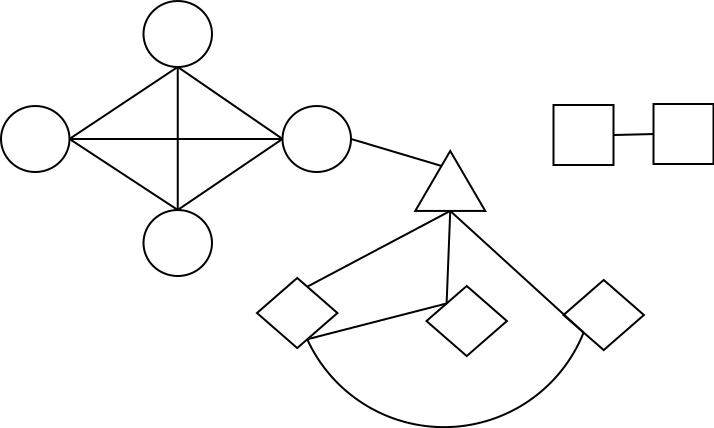
\includegraphics[width=0.7\textwidth]{figures/grafo.png}
\caption{O exemplo de teste triângulo está ligada ao grafo formado pela classe dos círculos e dos losangos, porém não apresenta ligações com os quadrados.}
\label{fig::grafo}
\end{figure}

%Para cada grafo representando uma classe, podemos calcular a credibilidade do exemplo de teste para aquela classe e a incorporar ao classificador Bayesiano. Decidimos modificar a Equação~\ref{eqn::classindependence}, sugerindo a seguinte fórmula:

%\begin{equation}\label{eqn::nbcredgrafo}
%P(X|c_{j}) = \prod^{D}_{i=1}{(P(x_i|c_j)) \cdot (\alpha + Cr_{rel}(X,c_j)) } 
%\end{equation}

%Como na Equação~\ref{eqn::classindependence}, continuamos calculando o produtório dos atributos que compõem o exemplo $X$, porém calculamos também a credibilidade de $X$ em relação a classe $c_i$. Utilizamos um fator $\alpha$ para evitarmos que a falta de uma aresta entre $X$ e o exemplo da classe $i$ possa resultar em uma probabilidade nula de que $X$ seja da classe $i$. 

Note que podemos, sem problema algum, juntar as Equações \ref{eqn::nbcred_attr} e \ref{eqn::nbcredgrafo} dando origem a um classificador Bayesiano que leva em conta tanto a credibilidade dos atributos quanto a dos relacionamentos:

\begin{equation}\label{eqn::nbcredcompleta}
P(X|c_{j}) = \prod^{D}_{i=1}{(P(x_i|c_j) \cdot Cr_{atr}(x_i,c_j)) \cdot (\alpha + Cr_{rel}(X,c_j)) } 
\end{equation}

A credibilidade dos atributos é calculada a partir dos relacionamentos e existe mesmo sem um exemplo de treinamento, porém, a credibilidade dos relacionamentos somente existe quando temos um exemplo de teste específico. Isso faz com que essa seja uma técnica \textit{lazy}, ou seja, somente utilizamos o conhecimento aprendido a partir dos relacionamentos quando estamos testando, sem a criação de um modelo previamente provido com o treinamento. 

Pelo fato de modelarmos os relacionamentos existentes entre os exemplos por meio de grafos, decidimos utilizar as diversas métricas da área de Redes Complexas (\cite{Newman03}) a fim de explorarmos as propriedades dos grafos criados. Um exemplo simples de uma dessas métricas é contar o número de vizinhos de um vértice, $viz(v,c_j)$. Essa função retorna o número de conexões  que o vértice $v$ tem com seus vizinhos que são da classe $c_j$. Partimos do pressuposto que se um vértice for importante para uma determinada classe $j$, $viz(v,c_j)$, será um valor superior para aquela classe. Na Figura~\ref{fig::grafo}, a classe \textit{Losango} seria a de maior credibilidade para classificarmos o triângulo, baseando nessa métrica. Outras várias métricas importantes podem ser listadas e combinada, sendo assim, atribuímos toda a Seção~\ref{sec::pg_cred_baseada_grafos} para maiores detalhes.  


